\documentclass[tikz,margin=3mm]{standalone}
\usetikzlibrary{trees}
\usepackage{tikz}


\begin{document}
    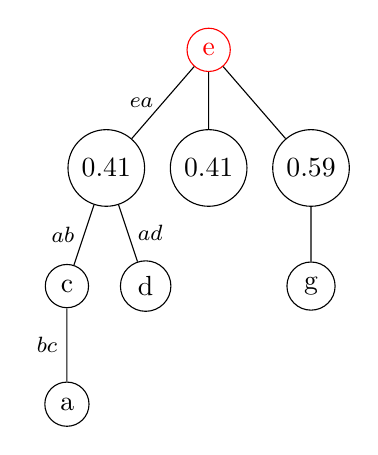
\begin{tikzpicture}[
   level distance = 1.5cm,
   level 1/.style = {sibling distance=1.3cm},
   level 2/.style = {sibling distance=1.0cm},
   level 3/.style = {sibling distance=0.8cm},
every node/.style = {circle,draw},
       lbl/.style = {rectangle, draw=none, #1,% position
                     font=\footnotesize}
                        ]
%
\node (Root) [red] {e}
    child {node {0.41}
        child {node {c}
            child {node {a}
            edge from parent node[lbl=left] {$bc$}
            }
        edge from parent node[lbl=left] {$ab$}
       }
    child {node {d}
    edge from parent node[lbl=right] {$ad$}
        }
    edge from parent node[lbl=left] {$ea$}
      }
    child { node {0.41}}
    child { node {0.59}
        child { node {g} }
          };
    \end{tikzpicture}

    \pagebreak

    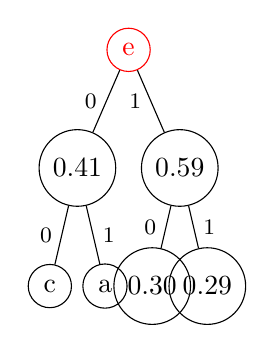
\begin{tikzpicture} [
        level distance = 1.5cm,
        level 1/.style = {sibling distance=1.3cm},
        level 2/.style = {sibling distance=0.7cm},
        level 3/.style = {sibling distance=0.8cm},
        level 4/.style = {sibling distance=0.7cm},
        level 5/.style = {sibling distance=0.6cm},
        level 6/.style = {sibling distance=0.5cm},
        every node/.style = {circle,draw, minimum size=0.1em},
        lbl/.style = {rectangle, draw=none, #1,% position
                     font=\footnotesize}
    ]
    
    \node (Root) [red] {e} {
            child {node {$0.41$} 
            child {node{c} edge from parent node[lbl=left] {$0$}} 
            child {node{a} edge from parent node[lbl=right] {$1$}}
            edge from parent node[lbl=left] {$0$}}
            child {node {0.59} 
            child {node{0.30} edge from parent node[lbl=left] {$0$}} 
            child {node{0.29} edge from parent node[lbl=right] {$1$}}
            edge from parent node[lbl=left] {$1$}}
    };

    \end{tikzpicture} 

    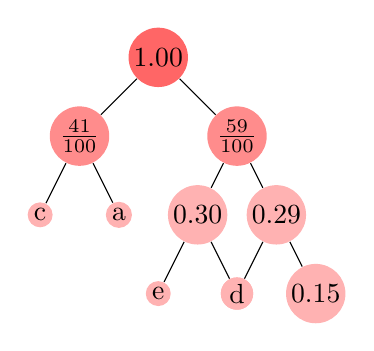
\begin{tikzpicture}
        [level distance=10mm,
        every node/.style={fill=red!60,circle,inner sep=1pt},
        level 1/.style={sibling distance=20mm,nodes={fill=red!45,}},
        level 2/.style={sibling distance=10mm,nodes={fill=red!30}},
        level 3/.style={sibling distance=5mm,nodes={fill=red!25,}}
        lbl/.style = {rectangle, draw=none, #1,% position
                     font=\footnotesize}]
        \node {1.00}
            child {node {$\frac{41}{100}$}
                child {node {c}}
                child {node {a}}
            }
            child {node {$\frac{59}{100}$}
            child {node {0.30}
            child {node {e}}
            child {node {b}}}
            child {node {0.29}
            child {node {d}}
            child {node {0.15}}}
        };
        \end{tikzpicture}

        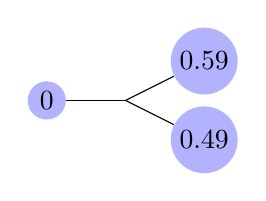
\begin{tikzpicture}[level distance=10mm,
            sibling distance=10mm,
            every node/.style={fill=blue!30,circle,inner sep=2pt},
            arrow/.style={edge from parent/.style={draw,-latex}}
          ]
          
          \node {0}
          child[grow=right] {
          child {node{0.49}} child {node{0.59}}
          };
          \end{tikzpicture}
          

\end{document}